\documentclass[10pt,twocolumn,letterpaper]{article}
\usepackage[T1]{fontenc}
\usepackage[utf8]{inputenc}
\usepackage{amsmath,amssymb,amsthm,mathtools,bm,braket}
\usepackage{mathptmx}
\renewcommand{\ttdefault}{pcr}
\usepackage[margin=0.68in,columnsep=0.26in,headheight=14pt,headsep=0.15in,footskip=0.28in]{geometry}
\usepackage{graphicx,booktabs,array,tabularx,longtable,multirow}
\usepackage{microtype,fancyhdr,caption,titlesec,enumitem,float,placeins}
\usepackage[most]{tcolorbox}
\usepackage[hidelinks,bookmarksnumbered=true,hypertexnames=false]{hyperref}
\usepackage{xurl}
\setlength{\parindent}{1em}
\setlength{\parskip}{0.16em}
\setlength{\emergencystretch}{2em}
\setlength{\abovedisplayskip}{6pt plus2pt minus2pt}
\setlength{\belowdisplayskip}{6pt plus2pt minus2pt}
\captionsetup{font=small,labelfont=bf,justification=raggedright,singlelinecheck=false}
\titleformat{\section}{\large\bfseries}{\thesection.}{0.45em}{}
\titleformat{\subsection}{\normalsize\bfseries}{\thesubsection}{0.45em}{}
\titleformat{\subsubsection}{\normalsize\bfseries}{\thesubsubsection}{0.45em}{}
\titlespacing*{\section}{0pt}{11pt plus2pt minus2pt}{5pt}
\titlespacing*{\subsection}{0pt}{8pt plus2pt minus2pt}{3pt}
\pagestyle{fancy}\fancyhf{}
\fancyhead[L]{\footnotesize SAM Volume I | Chapter \ChapterRoman}
\fancyhead[R]{\footnotesize Brady | Edition of 25 October 2026}
\fancyfoot[C]{\footnotesize\thepage}
\renewcommand{\headrulewidth}{0.3pt}
\newtheorem{theorem}{Theorem}[section]
\newtheorem{proposition}{Proposition}
\newtheorem{lemma}[theorem]{Lemma}
\newtheorem{corollary}[theorem]{Corollary}
\theoremstyle{definition}
\newtheorem{definition}[theorem]{Definition}
\newtheorem{assumption}[theorem]{Assumption}
\newtheorem{example}[theorem]{Example}
\theoremstyle{remark}
\newtheorem{remark}[theorem]{Remark}
\newcommand{\dd}{\mathrm{d}}
\newcommand{\ii}{\mathrm{i}}
\newcommand{\Tr}{\operatorname{Tr}}
\newcommand{\Span}{\operatorname{span}}
\allowdisplaybreaks[2]
\raggedbottom
\pdfmapfile{+cm.map}
\pdfmapfile{+cmextra.map}
\pdfmapfile{+symbols.map}
\pdfmapfile{+psnfss.map}
\pdfmapfile{+utm.map}
\pdfmapfile{=ps2pk35.map}
\pdfmapfile{+rsfs.map}

\newcommand{\ChapterRoman}{Supplement}
\hypersetup{pdftitle={SAM Volume I: Supplement: retired targets (Chapter X of the 19 October 2026 edition)},pdfauthor={Sean Brady}}
\begin{document}
\fancyhead[L]{\footnotesize SAM Volume I | Supplement}
\twocolumn[{
\begin{center}
{\small SAM VOLUME I\par}
\vspace{0.4em}
{\LARGE\bfseries Supplement: retired targets (Chapter X of the 19 October 2026 edition)\par}
\vspace{0.4em}
{\large Supplement to Volume I\par}
\vspace{0.5em}
{\large Sean Brady\par}
{\small Originator and conceptual director\par}
{\small Research development with OpenAI ChatGPT and Codex\par}
{\small Edition of 25 October 2026 (text of the unified expanded edition, 19 October 2026)\par}
\end{center}
\begin{minipage}{0.97\textwidth}\noindent\textbf{Abstract.} This supplement retains, unchanged in text and in their original section numbering, the parts of the 19 October 2026 edition of Volume I that the 25 October 2026 edition retires from the body of the volume on Sean Brady's decision: the whole of Chapter X on many-source accumulation and galaxy halos. Chapter XII Sections 6 and 9--19, retired with it under Option A, returned to the body of the volume later the same day on Sean Brady's decision: Section 6 to Chapter XII, Sections 9--19 as the new Chapter XIII.\end{minipage}
\vspace{0.9em}}]


\part*{Chapter X of the 19 October 2026 edition: Many-source accumulation and galaxy halos}
\noindent\textit{Abstract of the retained chapter.} This chapter develops the many-source accumulation account of galaxy support. It preserves the reported SPARC results while separating potential lifts, radial force, and geometry-dependent mass inference. The proposed coordinate $10/\pi$ is analyzed as a population identification, with explicit treatment of selection history, uncertainty, and the algebraic dependence of the mass-ratio statistic. A radial organization law and an untouched-sample test remain necessary for a predictive halo theory. The reported support deficit, radial randomization results, and outer mass assignment are preserved with their original receipt identifiers. New derivations expose which results share the same underlying statistic, quantify the approximate resolution of the population median, and constrain admissible radial profiles through density positivity. Disk geometry, stellar mass-to-light ratios, correlated observational uncertainties, and the distinction between measured-radius and virial masses are treated explicitly. The constituent interpretation is kept separate from the gravitational support measurement. No SPARC replay or new halo-formation simulation is claimed; the chapter ends with a prospective protocol and falsifiable requirements for a completed organization law.

\section{Inventory is not a halo profile}

A cosmic inventory specifies how much of a component exists on average. A rotation curve specifies the radial gravitational support required in one galaxy. Connecting them requires a distribution law. The identity $\Omega_c=\Omega_m-\Omega_b$ cannot, by itself, determine a halo radius, a central density, a concentration, or the relation between a halo and its baryonic disk. This chapter develops the original many-source accumulation proposal while making that missing dynamical step explicit.

The empirical starting point is the supplied chapter's analysis of SPARC, a public compilation of 175 late-type galaxies with infrared photometry and resolved rotation curves [X.1]. The reported campaign finds a large baryonic support deficit, a radial rise in a dimensionless support ratio, and an outer population centre near $10/\pi$. It also reports a near-unity median for masses assigned with that coordinate. These results are preserved as historical receipts. The underlying galaxy tables, cuts, randomization code, and profile parameters were not supplied with this expansion; no independent SPARC reanalysis is claimed.

Three questions must remain distinct. Does a support deficit exist under the adopted stellar population and geometry assumptions? Does the selected ratio summarize its population centre? Does a substrate transport law predict the radial profile and its galaxy-to-galaxy variation? The first two are empirical or phenomenological questions addressed by the retained campaign. The third is the outstanding physical closure. Identifying these levels prevents a successful descriptive coordinate from being presented as a completed theory of galaxy formation.

The symbol $X_\infty$ is retained for continuity with the original draft, but its present empirical meaning is an outer-sample coordinate. It has not been established as the mathematical limit $r\to\infty$ of each galaxy. This distinction becomes essential when considering finite baryonic mass and approximately flat rotation curves.

\section{The many-source field and the force readout}
\subsection{Linear lifts and their continuum limit}

The weak-field proposal adds source lifts,
\begin{equation}
 A_{\rm lift}(\mathbf x)=\sum_i\frac{2GM_i}{c^2|\mathbf x-\mathbf x_i|},\qquad
 A_{\rm lift}(\mathbf x)=\frac{2G}{c^2}\int
 \frac{\rho(\mathbf x')}{|\mathbf x-\mathbf x'|}\,d^3x'.
 \label{c10:lift}
\end{equation}
The second expression assumes a continuum density for which the integral is defined, with an appropriate boundary or background subtraction. An infinite homogeneous universe cannot be inserted into an isolated-system potential integral without specifying that subtraction. For the present galaxy calculation the kernel is an isolated weak-field adapter, not a derivation of cosmological boundary conditions.

Under the Newtonian identification $\Phi=-c^2A_{\rm lift}/2$, circular motion in an axisymmetric midplane obeys
\begin{equation}
 V_c^2(R)=R\frac{\partial\Phi(R,0)}{\partial R}
 =-\frac{c^2R}{2}\frac{\partial A_{\rm lift}(R,0)}{\partial R}.
 \label{c10:force}
\end{equation}
This equation exposes an important distinction obscured by calling every accumulation quantity simply $A$. Circular support is determined by a derivative of the potential-like lift. It is not generally the value of that lift. A useful dimensionless force account is therefore
\begin{equation}
 A_{\rm circ}(R)\equiv\frac{2V_c^2(R)}{c^2}
 =-R\,\partial_R A_{\rm lift}(R,0).
 \label{c10:acirc}
\end{equation}
For a point mass, the derivative restores the familiar $2GM/(c^2R)$, so the two expressions coincide. That special coincidence must not be generalized without checking the mass geometry.

\subsection{A spherical identity and its proof}

For a spherical density with finite exterior potential, the lift can be written
\begin{equation}
 A_{\rm lift}(r)=\frac{2G}{c^2}\left[
 \frac{M(<r)}{r}+\int_r^\infty4\pi r'\rho(r')\,dr'\right].
 \label{c10:sphericallift}
\end{equation}
Differentiate the bracket. The derivative of $M/r$ contains $M'/r-M/r^2$. Since $M'=4\pi r^2\rho$, the derivative of the exterior-shell integral cancels the $M'/r$ term. Consequently,
\begin{equation}
 A_{\rm circ}(r)=\frac{2GM(<r)}{c^2r},\qquad
 V_c^2(r)=\frac{GM(<r)}{r}.
 \label{c10:spherical}
\end{equation}
This proves the original cumulative support reading under spherical symmetry and the Newtonian adapter. It also shows why exterior shells may contribute to the lift while contributing no radial force. The enclosed account in Eq.~\eqref{c10:spherical} is a force-derived quantity, not the full potential in Eq.~\eqref{c10:sphericallift}.

The superposition law is linear in prescribed source density. It does not determine that density. A linear Green function supplies the response to a source; a halo-formation law must explain the source's distribution, its conservation, and its equilibrium or time evolution. This is the central dependency of the chapter. Summing known baryonic lifts cannot create an unspecified nonbaryonic component merely by changing notation.

\section{What the rotation-curve decomposition measures}

Let $V_{\rm obs}$ denote the inferred circular speed after the observational analysis, and let the baryonic model supply gas, disk, and bulge contributions. With consistent force signs,
\begin{align}
 V_{\rm bar}^2&=V_{\rm gas}^2+\Upsilon_dV_{\rm disk}^2
 +\Upsilon_bV_{\rm bulge}^2,\label{c10:baryons}\\
 V_{\rm h}^2&=V_{\rm obs}^2-V_{\rm bar}^2,\qquad
 X=\frac{V_{\rm h}^2}{V_{\rm bar}^2},\qquad
 f_{\rm supp}=\frac{X}{1+X}.
 \label{c10:x}
\end{align}
Here $\Upsilon_d$ and $\Upsilon_b$ are stellar mass-to-light ratios at the specified observing band. The original convention is $\Upsilon_d=0.5$ at $3.6\,\mu\mathrm m$. It does not print a numerical bulge value, so the expanded chapter does not invent one. That value, including treatment of galaxies without bulges, belongs in the campaign manifest.

The squared-component notation conventionally means a signed contribution to radial force. In regions where a component's geometry produces an outward radial contribution, the tabulated signed convention must be respected; squaring a signed speed without restoring its force sign is incorrect. The total baryonic radial acceleration must be positive where $X$ is interpreted as the ratio in Eq.~\eqref{c10:x}.

A negative residual $V_{\rm h}^2$ can arise from measurement uncertainty, an inappropriate stellar normalization, noncircular motion, or model inadequacy. It should not be silently clipped to zero and then omitted from logarithmic statistics. The analysis must specify its handling before examining the desired median. The difference between the original 175-galaxy sample and the 173-galaxy mass-ratio sample is therefore part of the result: the supplied text states only that 173 have nonzero measured halo mass, not the full exclusion rule or the identities and reasons for the two omissions.

The quantity $f_{\rm supp}$ is exactly a \emph{fraction of modeled circular support}. It is a physical enclosed mass fraction only when the conversion from speed to mass is valid for both components in the stated geometry. In a disk-plus-spherical-halo model, the halo mass $rV_h^2/G$ can be meaningful, while $rV_{\rm bar}^2/G$ is generally an equivalent spherical baryonic mass rather than the true disk mass inside $r$. This distinction does not invalidate the support ratio; it prevents a geometrical overinterpretation.

\section{The reported deficit and the clustering requirement}

The original campaign reports three successive results. CR022@08 finds nonzero many-source accumulation wherever matter is present. CR024@08 uses 175 galaxies and 3,391 measured points and finds a median outer support fraction $0.760699$. Its bounded post-Big-Bang compact or trapped-field subchannel supplies only $2.58\%$ of the residual in that account. CR025@08 introduces a clustered profile and reports a median rotation-curve RMS falling from $40.95$ to $3.63\,\mathrm{km\,s^{-1}}$, with median overdensity about $7.9\times10^4$ relative to the cosmic dark-component mean.

These are distinct conclusions. The bounded subchannel result excludes that specific allocation as a sufficient explanation within its assumptions; it does not exclude every possible post-formation mechanism. The improved RMS shows that the chosen clustered profile can supply the missing support; without its explicit parameters, priors, and fitting procedure, it does not establish parameter-free predictive accuracy. The profile itself must be published before the improvement can be compared fairly with alternative halo descriptions.

A simple calculation explains why a homogeneous cosmic component is insufficient on galactic scales under ordinary gravity. If its density is $\bar\rho_c=\Omega_c\rho_{\rm crit}$, then
\begin{equation}
 \begin{gathered}
 M_c(<r)=\frac{4\pi}{3}\bar\rho_c r^3,\qquad V_c^2(r)=\frac{\Omega_cH_0^2r^2}{2},\\
 V_c=H_0r\sqrt{\frac{\Omega_c}{2}}.
 \end{gathered}
 \label{c10:uniform}
\end{equation}
This is a local spherical estimate, not a treatment of a homogeneous background as an isolated bound halo. For illustrative values $H_0=67.25\,\mathrm{km\,s^{-1}\,Mpc^{-1}}$, $\Omega_c=0.27$, and $r=20\,\mathrm{kpc}$, it yields about $0.49\,\mathrm{km\,s^{-1}}$. The assumptions and arithmetic, rather than a new galaxy observation, establish the scale mismatch. Raising the contribution to galactic speeds requires a substantial overdensity, an altered force law, or both.

If the model retains the weak-field kernel, clustering is therefore necessary. It is not sufficient: an arbitrarily chosen clustered density can fit many curves. The scientific question is whether the source observables and a common physical law select the required density before the rotation speeds are used to determine it.

\begin{figure*}[t]
\centering
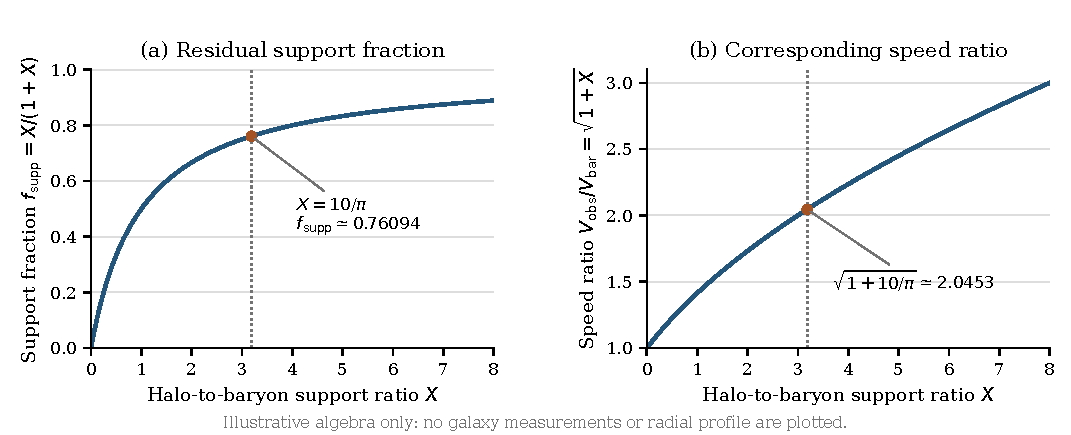
\includegraphics[width=\textwidth]{figures/ch10_support_mapping.pdf}
\caption{Illustrative algebra of the halo-to-baryon circular-support coordinate, $X=V_h^2/V_{\rm bar}^2$, for positive baryonic support and nonnegative residual support. (a) The residual fraction is $f_{\rm supp}=X/(1+X)$. (b) The corresponding speed ratio is $V_{\rm obs}/V_{\rm bar}=\sqrt{1+X}$. The marked count-selected coordinate $10/\pi$ maps to $f_{\rm supp}\simeq0.76094$ and a speed ratio of approximately $2.0453$. No galaxy data, empirical scatter, radial profile or fitted trend is shown. A support fraction is an enclosed mass fraction only under the geometry assumptions needed for that conversion.}
\label{fig:c10:supportmapping}
\end{figure*}

\section{Radial organization and the reported permutation tests}

CR031 and its appeal CR031b compute $X(r)$ at measured radii and bin the result in $u=r/R_{\rm out}$. The retained summary reports a median rising from baryon-dominated interiors toward an outer value near $3.12$, an inner-to-outer change $+1.971$, and a logarithmic-spread contraction $0.218$. The exact spread definition and binning rule need to accompany a reproduction; a change in a logarithmic width is not necessarily a change in an ordinary standard deviation.

Two null families, each with 1,000 seeded trials, are reported. Within-galaxy radial shuffles remove the original ordering of support values in each galaxy. Galaxy-randomized normalized radii remove the original cross-galaxy radial alignment. No randomized trial reaches the canonical statistic. With the conventional plus-one Monte Carlo correction,
\begin{equation}
 \widehat p=\frac{b+1}{B+1}=\frac{1}{1001},\qquad b=0,\ B=1000.
 \label{c10:permutation}
\end{equation}
This is the finite-randomization reporting floor, not proof that the underlying tail probability equals exactly $1/1001$. A Monte Carlo estimate also has sampling uncertainty. Valid calibration requires exchangeability under the proposed null and a statistic fixed before inspecting the randomized results.

The original CR031 used a binary kill-fraction score and returned BOUNDARY; CR031b rescored the same trials using a continuous statistic. Preserving both is appropriate. The revised statistic can reveal information discarded by a binary score, but a statistic chosen after looking at results requires its selection history to be disclosed. A new independent validation should freeze that statistic before generating its null ensemble.

These tests address radial structure under specified randomizations. They do not test the numerical identity $10/\pi$, establish a particular physical mechanism, or compare SAM with a realistic galaxy-formation model. Observed radii are not exchangeable under many physically motivated alternatives, so a shuffle that destroys a general galaxy trend is not a complete competing theory. The two $p$ values should not be multiplied as though independent: both are derived from the same galaxies and related support measurements.

Normalized radius also introduces selection effects. $R_{\rm out}$ is the last measured radius, determined partly by sensitivity, gas extent, angular resolution, inclination, and data quality. It is not necessarily a common multiple of a physical halo radius. A trend in $r/R_{\rm out}$ should be checked beside trends in disk scale lengths, absolute radius, and baryonic acceleration. Those checks can distinguish a universal physical organization from an alignment enhanced by the observing window.

\section{The coordinate \texorpdfstring{$10/\pi$}{10/pi} and its actual precision}

The proposed outer coordinate is
\begin{equation}
 X_\infty=(\mathcal R-\widehat h)\Omega_m
 =\frac{12-2}{\pi}=\frac{10}{\pi}=3.18309886\ldots,
 \label{c10:coordinate}
\end{equation}
where $\mathcal R$ is the radix and $\widehat h$ the binary arity. Under the support-fraction mapping,
\begin{equation}
 f_\infty=\frac{X_\infty}{1+X_\infty}
 =\frac{10}{\pi+10}=0.76094278\ldots.
 \label{c10:fraction}
\end{equation}
The campaign reports an empirical plateau $3.18$ in CR025 and a binned median $3.12$ in CR031b. Its raw outer support-fraction median is $0.760699$. These numbers are compatible at the resolution of the sample, but they are not one interchangeable estimator: a binned median, a raw galaxy median, and a fitted plateau can weight the data differently.

CR033 calculated the coordinate from the substrate atoms behind a file guard excluding earlier branch results. The source also states that the identity was proposed after the empirical plateau had been measured. The guard establishes a restricted execution dependency; it cannot make the earlier human or programmatic selection prospective. The appropriate description is a structural identification of a known empirical centre. The phrase ``no continuous per-galaxy adjustment'' is defensible for the later evaluation; ``no selection freedom'' is not.

The closing review correctly emphasizes statistical resolution. Suppose, only as an approximation, that independent galaxy values of $y=\log_{10}X$ are Gaussian with standard deviation $s=0.38$ dex and sample size $n=173$. The asymptotic variance of a sample median is $1/[4n p(y_0)^2]$. Inserting the Gaussian density at its centre gives
\begin{equation}
 \operatorname{SE}(\widetilde y)\simeq
 \sqrt{\frac{\pi}{2}}\frac{s}{\sqrt n}
 \simeq0.0362\ \mathrm{dex}.
 \label{c10:medianerror}
\end{equation}
A linearized fractional uncertainty is $\ln(10)\operatorname{SE}(\widetilde y)\simeq8.3\%$; converting one positive logarithmic standard error exactly gives about $8.7\%$. These are two conventions for the same approximate scale, not conflicting uncertainty estimates.

Differentiating $f=X/(1+X)$ with respect to $y$ gives
\begin{equation}
 \frac{df}{dy}=\ln(10)\frac{X}{(1+X)^2},\qquad
 \operatorname{SE}(\widetilde f)\simeq0.0152.
 \label{c10:ferror}
\end{equation}
The review rounds this scale to about $0.016$. The numerical difference between $0.760943$ and $0.760699$ is only about $0.016$ of the linearized standard error. Four-decimal agreement therefore carries no four-decimal evidential precision. Moreover, the calculation assumes independent Gaussian log scatter; a galaxy bootstrap, measurement-error model, and systematic uncertainties are needed for a defensible interval. The formula is a diagnostic, not a replacement for that analysis.

\section{The mass-placement result and its dependence on the plateau}

For a spherical halo, the selected coordinate supplies an outer mass assignment,
\begin{equation}
 M_{h,{\rm pred}}(<R_{\rm out})=
 \frac{R_{\rm out}X_\infty V_{\rm bar}^2(R_{\rm out})}{G}.
 \label{c10:massplacement}
\end{equation}
The original results for the 173-galaxy subset are a median predicted/measured ratio $0.9983$ for the empirical value $3.18$ (CR032), and $0.99928$ for $10/\pi$ (CR033), evaluated against a reported precommitted $\pm12\%$ tolerance. The reported scatter is approximately $0.38$ dex. That scatter is a factor $10^{0.38}\simeq2.40$ multiplicatively, far larger than the difference of the median from unity.

The following algebra determines what independent information this test contains. If the measured halo mass uses the same outer speed residual and spherical conversion,
\begin{equation}
 M_{h,{\rm obs}}=\frac{R_{\rm out}[V_{\rm obs}^2-V_{\rm bar}^2]}{G},
 \qquad \frac{M_{h,{\rm pred}}}{M_{h,{\rm obs}}}
 =\frac{X_\infty}{X(R_{\rm out})}.
 \label{c10:ratioidentity}
\end{equation}
The radius, gravitational constant, and baryonic speed normalization cancel except through the already-defined $X$. For an odd sample with positive values and the usual order-statistic median, monotonic inversion implies
\begin{equation}
 \operatorname{med}\!\left(\frac{X_\infty}{X_i}\right)
 =\frac{X_\infty}{\operatorname{med}(X_i)}.
 \label{c10:medianidentity}
\end{equation}
The proof is simply that sorting positive $X_i$ reverses their order under inversion, leaving the middle index in the middle. Thus a near-unity median mass ratio on the same selected sample is principally a restatement of agreement with its outer support-ratio median. It is a useful consistency check and a way to express the scale in mass units, but not an independent prediction of 173 halo masses.

For even samples, interpolated medians require care because averaging and nonlinear transformation need not commute. Nonpositive residuals and different weighting conventions also break the simple statement. These are reasons to publish the estimator, not reasons to disregard the cancellation. A genuinely independent mass test could use a different gravitational observable with its own geometry and errors, or a prospective rotation-curve sample untouched during selector construction.

For the draft's illustrative galaxy, $V_{\rm bar}=100\,\mathrm{km\,s^{-1}}$ at $R_{\rm out}=20\,\mathrm{kpc}$, with $G=4.30091\times10^{-6}\,\mathrm{kpc}\,(\mathrm{km\,s^{-1}})^2M_\odot^{-1}$, the equivalent baryonic mass is $4.65\times10^{10}M_\odot$. Equation~\eqref{c10:massplacement} gives $1.48\times10^{11}M_\odot$, and the associated speed is
\begin{equation}
 V_{\rm pred}=V_{\rm bar}\sqrt{1+X_\infty}
 \simeq204.5\,\mathrm{km\,s^{-1}}.
 \label{c10:example}
\end{equation}
These are arithmetic consequences of the assumed coordinate and illustrative inputs. They are not an additional observed galaxy or a native dynamical run.

\section{Disk geometry and stellar-population sensitivity}

A thin exponential disk makes the spherical approximation's limitation explicit. For surface density $\Sigma(R)=\Sigma_0e^{-R/R_d}$, its mass inside cylindrical radius $R$ is
\begin{equation}
 M_d(<R)=2\pi\Sigma_0R_d^2[1-e^{-u}(1+u)],\quad u=R/R_d.
 \label{c10:diskmass}
\end{equation}
The midplane speed is instead given by the disk Green function; for the ideal exponential disk [X.3],
\begin{equation}
 V_d^2=4\pi G\Sigma_0R_d y^2
 [I_0(y)K_0(y)-I_1(y)K_1(y)],\quad y=R/(2R_d).
 \label{c10:freeman}
\end{equation}
The modified Bessel functions encode the force from material both inside and outside the cylindrical radius. Define $q_d=RV_d^2/[GM_d(<R)]$. Equation~\eqref{c10:freeman} does not reduce to $q_d=1$ at every radius. Therefore a spherical ``baryonic mass'' inferred from the disk speed is radius-dependent relative to the actual disk mass.

The correct comparison does not require abandoning the support ratio. It requires retaining the disk force computed from photometry and using a separately stated halo geometry when turning the residual into halo mass. A finite-thickness disk, gas distribution, and bulge add their own kernels. Using SPARC's disk-based component speeds is already different from assuming a spherical baryon distribution; an additional geometry correction must not double-count the correction contained in those components.

The dependence on stellar mass-to-light ratio can be derived without a new data run. Write $B=V_{\rm bar}^2$ and $D=V_{\rm disk}^2$, holding the observed speed and other components fixed. Then
\begin{equation}
 \frac{\partial X}{\partial\Upsilon_d}
 =-\frac{V_{\rm obs}^2D}{B^2},\qquad
 \frac{\partial f_{\rm supp}}{\partial\Upsilon_d}
 =-\frac{D}{V_{\rm obs}^2}.
 \label{c10:upsderivative}
\end{equation}
Increasing stellar mass lowers the inferred missing support, as expected. The effect differs across galaxies because disk, gas, and bulge contributions differ. A common $\Upsilon_d$ shift is a population systematic; it does not average away like independent velocity noise. A required robustness product is therefore the median mass ratio and scatter as functions of $\Upsilon_d$, with a declared literature-motivated range and bulge policy.

Distance and inclination also matter. At fixed angular photometry, baryonic model speeds generally scale with adopted distance, whereas inclination affects deprojected observed speeds strongly for nearly face-on disks. These uncertainties are correlated within a galaxy across radii. Treating thousands of radial points as independent measurements of one global coordinate would produce an artificially small uncertainty. The galaxy, rather than the radial point, is the natural top-level resampling unit for a population median.

\section{What a radial law must accomplish}

A valid organization law must map source observables and stated initial or boundary conditions to $X(r)$ or $\rho_h(r)$ without using the target rotation curve to set an undisclosed profile parameter. It must conserve the relevant inventory, explain its concentration, allow galaxy diversity, and yield an admissible density. Even within the spherical adapter, positivity gives a nontrivial constraint:
\begin{equation}
 \rho_h(r)=\frac{1}{4\pi Gr^2}
 \frac{d}{dr}\left[rX(r)V_{\rm bar}^2(r)\right]\geq0.
 \label{c10:densitytest}
\end{equation}
An arbitrary smooth rise toward a plateau can violate this condition if the baryonic force falls too rapidly. Smoothness and visual agreement are not enough. The derivative condition should be checked together with finite enclosed mass and the intended outer boundary.

A constant $X$ at arbitrarily large radii has a particularly clear consequence. Outside a finite baryonic distribution, $V_{\rm bar}^2\sim GM_b/r$. If $X\to X_\infty<\infty$, then $V_{\rm obs}^2\sim(1+X_\infty)GM_b/r$, which declines in the Keplerian manner. Conversely, an indefinitely flat observed curve with finite baryonic mass would require $X\propto r$. The two asymptotic statements cannot both hold. This proves why the currently observed outer-sample centre should not be promoted to an infinite-radius saturation theorem.

A candidate equilibrium or transport law should state its physical content before presenting a fitted formula. A collisionless component needs a phase-space distribution and a dynamical equation. A pressure-supported effective medium needs a stress relation and stability criteria. A dissipative component needs an energy-loss and heating account. A population of compact objects needs its formation, mass spectrum, relaxation, and accretion assumptions. Calling these alternatives ``trapped-A'' does not choose among them.

For example, the spherical equilibrium identity $d(\rho\sigma_r^2)/dr+2\beta\rho\sigma_r^2/r=-\rho\,d\Phi/dr$ would introduce a velocity-dispersion profile and an anisotropy $\beta$. It is a possible bookkeeping framework, not a SAM-derived closure. Unless those additional functions are supplied by a physical law or constrained independently, writing the equilibrium equation merely relocates the freedom. The same caution applies to a diffusion equation with an unspecified diffusion coefficient or a source term chosen to recover the desired profile.

\section{Comparators, constituents, and independent constraints}

A fair comparison distinguishes a single population coordinate from a full radial model. The NFW family uses a scale density and scale radius,
\begin{equation}
 \rho_{\rm NFW}(r)=\frac{\rho_s}{(r/r_s)(1+r/r_s)^2},
 \label{c10:nfw}
\end{equation}
while a cored Burkert family can be written
\begin{equation}
 \rho_{\rm B}(r)=\frac{\rho_0}{(1+r/r_0)[1+(r/r_0)^2]}.
 \label{c10:burkert}
\end{equation}
These are specified profile families [X.4--X.5]; their effective freedom depends on which scaling relations or priors are imposed. A numerical comparison must count those assumptions alongside stellar mass-to-light ratio, distance, and inclination policies. It would be misleading to compare a two-parameter full-curve fit with a one-number outer median and report only which has fewer named parameters.

The radial-acceleration relation uses the same physical accelerations, $g_{\rm obs}=V_{\rm obs}^2/r$ and $g_{\rm bar}=V_{\rm bar}^2/r$, so
\begin{equation}
 X=\frac{g_{\rm obs}}{g_{\rm bar}}-1.
 \label{c10:raridentity}
\end{equation}
The empirical relation reported by McGaugh, Lelli, and Schombert [X.2] is therefore a direct comparator for radial organization, not an unrelated cosmological test. Its commonly used interpolation is
\begin{equation}
 g_{\rm obs}=\frac{g_{\rm bar}}
 {1-\exp[-\sqrt{g_{\rm bar}/g_\dagger}]},
 \label{c10:rar}
\end{equation}
with a fitted acceleration scale $g_\dagger$. Its low-acceleration behavior implies $X\sim\sqrt{g_\dagger/g_{\rm bar}}$, rather than a universal constant for every outer point. A narrow population centre can still occur because a sample has a particular distribution of outer accelerations. Testing this possibility is necessary before interpreting the centre as a new universal capacity law.

The closing review contrasts roughly $0.1$ dex scatter for a radial-acceleration description with the present $0.38$ dex halo-mass-ratio scatter. These are not automatically commensurate residuals: the observables, cuts, weights, and propagated uncertainties differ. The proper response is to evaluate both prescriptions on the same data, in the same residual variable, using identical nuisance assumptions and holdout rules. That comparison remains to be performed; the raw scatter contrast alone is neither a fair rejection nor a validation.

Finally, gravitational support does not identify halo constituents. A viable compact-object account must specify the compact fraction, normalized mass function, spatial clustering, and the physical meaning of any noncompact trapped component. Microlensing, dynamical heating, accretion emission, and cosmological energy injection depend on those quantities [X.6]. A total halo density without a constituent prescription cannot be tested against them. Neither the support plateau nor a population median mass ratio establishes primordial black holes as the carrier of the dark inventory.

Chapter XII must supply the formation epoch and abundance for any proposed primordial component. Those results must be compatible with the thermal history and light-element tests of Chapter IX. No present-day allowed mass interval alone proves that the required objects form with the required abundance. In particular, an epoch relevant to heavy seeds can interact with nucleosynthesis, whereas a much lighter surviving population can require physics far earlier than the recombination lane covers. The dependence across chapters is a physical calculation still owed, not an interpretive bridge already crossed.

\section{A prospective test with explicit stopping rules}

The proposed CR034 test should freeze $10/\pi$, the stellar conventions, geometry, sample cuts, statistic, and uncertainty procedure before opening a genuinely untouched sample. A different survey name is insufficient if many of its galaxies or rotation measurements already occur in SPARC. Cross-matching objects and data provenance is part of protecting the holdout. Candidate surveys named in the original draft include THINGS, LITTLE THINGS, and PROBES; no claim is made here that any particular subset is untouched.

The primary observable should be specified in advance. For an outer-support test, use one defined outer estimator per galaxy and retain failed or nonpositive residual cases under a declared rule. The primary statistic can be the median $\log_{10}[X_\infty/X_{\rm out}]$, but a median alone can conceal broad or systematic failure. Secondary diagnostics should include scatter, coverage, and residual trends with surface brightness, gas fraction, mass, scale length, outer acceleration, and radial extent. These diagnostics test whether a common centre is hiding distinct populations.

Measurement uncertainty should propagate by drawing correlated galaxy-level nuisance variables and velocity uncertainties, then recomputing the full estimator. Population uncertainty can be estimated by resampling galaxies. Shared photometric or stellar-population systematics require separate perturbations rather than independent draws for each point. The final interval should state which of these sources is included. The historical $\pm12\%$ criterion can be retained as a declared centre tolerance, but it must not be confused with a claim that individual halo masses are predicted to twelve percent.

A minimal failure rule is that the frozen coordinate falls outside the prespecified population interval or exhibits a prespecified systematic residual that the claimed universality forbids. A stronger radial-law claim must also predict the curve shape and its scatter without fitting hidden galaxy-specific parameters. If the holdout fails, selecting a new simple constant creates a new hypothesis; it does not rescue the original prospective test. If it passes, the result validates that population statistic on the tested domain, not automatically the constituent model or the whole cosmology.

The immediate completion priorities are therefore concrete: publish CR025's full profile and parameter origins; reproduce the support statistics with galaxy-level uncertainties; separate force accounts from potential lifts and true masses; test stellar and geometric sensitivity; and execute the frozen independent comparison. The present chapter supplies a coherent empirical coordinate and several analytic checks. The radial dynamical law remains the decisive missing ingredient.

\section{An inference ledger for the halo claim}

A useful way to organize the remaining work is to track which inference each observation can support. The observed line-of-sight velocities, distances, and inclinations first determine a kinematic rotation curve. Photometry and gas maps, combined with stellar assumptions and geometry, determine the baryonic contribution. Subtracting the two yields a residual acceleration. Choosing a halo shape converts that acceleration to a density or enclosed mass. Choosing a constituent model converts the density to a number of objects or an effective field state. Finally, a formation model connects that population to the early-universe inventory. Each arrow adds assumptions, and no agreement at an earlier arrow eliminates the later ones.

This ledger is especially important when discussing the phrase ``the halo is the cosmic inventory, clustered.'' Within a model that identifies the residual with nonbaryonic mass and retains the standard force law, the phrase is a sensible programmatic statement. It is not a measured identity between a local rotation-curve residual and the cosmological density fraction. The local baryon retention efficiency, material outside the measured radius, halo assembly, and selection of luminous disks all intervene. A universal cosmic ratio need not be the ratio inside the last observed radius of every galaxy.

There is also a distinction between an enclosed mass and a virial mass. Equation~\eqref{c10:massplacement} applies only inside $R_{\rm out}$ under the adopted halo geometry. It does not supply a mass at an overdensity radius such as $R_{200}$. Extrapolating to that radius requires the missing outer profile and a definition of the reference density. Any comparison with cosmological mass functions or abundance matching must therefore include the extrapolation rather than label the measured-radius mass simply ``the halo mass.''

A model with a correct population centre but unmodeled scatter can still be useful. It provides a baseline against which to ask whether residuals correlate with independent observables. If a concentration relation is later proposed to explain those residuals, it should be fitted on a training subset, frozen, and tested elsewhere. Repeatedly explaining the same residuals with new structural expressions would accumulate discrete model flexibility even if no continuous parameter appears in the final printed formula.

The most valuable next result would not be another decimal place in the median. It would be a demonstrated map from a galaxy's baryonic surface-density profile and specified formation information to its entire residual acceleration profile, together with an uncertainty distribution. Such a result would explain why galaxies with very different interiors exhibit the reported aggregate trend, state where the trend should fail, and distinguish a physical organization law from a convenient normalization. The present analytic identities identify exactly what that map must respect.

\section{Deriving a finite-disk force kernel}

The distinction between a potential-like lift and circular support can be developed directly for a disk. Take an axisymmetric surface density $\Sigma(R')$ confined to the plane $z=0$, with finite total mass. At a point $(R,z)$, the Newtonian potential is
\begin{equation}
 \begin{split}
 \Phi(R,z)=-G\int_0^\infty R'\,dR'\,\Sigma(R')
 \int_0^{2\pi}\frac{d\varphi'}{\sqrt{s}},\\
 s=R^2+R'^2-2RR'\cos\varphi'+z^2.
 \end{split}
 \label{c10:diskkernel}
\end{equation}
This follows from summing point-source potentials over rings, with area element $R'dR'd\varphi'$. It supplies a concrete many-source realization of Eq.~\eqref{c10:lift}. Differentiating before taking the midplane limit yields
\begin{equation}
 \begin{split}
 V_c^2(R,z)=GR\int_0^\infty R'\,dR'\,\Sigma(R')
 \int_0^{2\pi}\frac{R-R'\cos\varphi'}{s^{3/2}}\,d\varphi'.
 \end{split}
 \label{c10:diskforcekernel}
\end{equation}
The radial derivative is the essential operation. Rings outside the observation radius do not disappear as spherical shells do. In fact, sufficiently interior to an isolated ring, its net in-plane pull is outward. An enclosed-mass approximation discards precisely this geometrical information.

For a razor-thin disk the kernel has an integrable potential singularity at the source plane, while its differentiated form requires careful limiting or principal-value treatment. It is unsafe to evaluate a naïve point grid with a source exactly at the observation point. A finite-thickness density regularizes the local structure physically; a softened numerical kernel changes the physical model unless its scale is tied to that thickness and a convergence study is provided. These are practical requirements for a native many-source computation, not optional numerical details.

An alternative representation separates the vertical dependence through a Hankel transform. Define
\begin{equation}
 S(k)=\int_0^\infty R'\Sigma(R')J_0(kR')\,dR'.
 \label{c10:hankel}
\end{equation}
The axisymmetric solution of the thin-sheet Poisson problem can then be written
\begin{equation}
 \Phi(R,z)=-2\pi G\int_0^\infty
 S(k)J_0(kR)e^{-k|z|}\,dk.
 \label{c10:hankelpotential}
\end{equation}
One verifies the construction by applying the cylindrical Laplacian away from the plane and using the jump of the vertical derivative across the sheet. That jump is $4\pi G\Sigma$, as required by integrating Poisson's equation through the disk. Radial differentiation gives $V_c^2=2\pi GR\int kS(k)J_1(kR)\,dk$ in the midplane. The force and the mass integral are manifestly different transforms of the same surface density.

For $\Sigma=\Sigma_0e^{-R/R_d}$, the transform is
\begin{equation}
 S(k)=\frac{\Sigma_0R_d^2}{[1+(kR_d)^2]^{3/2}}.
 \label{c10:exponentialtransform}
\end{equation}
It can be obtained by differentiating the Laplace transform of $J_0$ with respect to the exponential decay constant. Substitution gives the Bessel-function disk result quoted earlier. This route makes clear which assumptions are responsible for that result: an infinitesimally thin exponential sheet, a Newtonian kernel, and axisymmetry. A different observed surface-density profile should be integrated directly rather than forced into an exponential solely because the analytic formula is convenient.

At radii much larger than a finite disk's extent, the leading potential is $-GM_d/r$ and the spherical force approximation becomes asymptotically valid. Near the disk scale length it need not be accurate. A useful geometry audit therefore reports the exact-kernel and spherical-equivalent forces as functions of radius, then propagates their difference through the same support estimator. It does not apply one global correction factor to all galaxies and radii.

\section{A positive-density radial example with no fitted galaxy data}

A complete radial function can be constructed analytically to illustrate the constraints on a future organization law. This is a conditional example, not a proposed derivation of the SAM halo profile. Choose a spherical baryonic model with enclosed mass
\begin{equation}
 M_b(<r)=M_b\frac{r^2}{(r+b)^2},\qquad
 V_{\rm bar}^2(r)=\frac{GM_br}{(r+b)^2},\quad b>0.
 \label{c10:toybaryons}
\end{equation}
Now stipulate a support ratio that rises from zero to the selected coordinate,
\begin{equation}
 X(r)=X_\infty\frac{r}{r+b}.
 \label{c10:toyx}
\end{equation}
Because both components are spherical in this example, multiplying enclosed baryonic mass by $X$ is legitimate. The halo mass and density are
\begin{equation}
 \begin{gathered}
 M_h(<r)=X_\infty M_b\frac{r^3}{(r+b)^3},\\
 \rho_h(r)=\frac{3X_\infty M_bb}{4\pi(r+b)^4}.
 \end{gathered}
 \label{c10:toydensity}
\end{equation}
The density follows by differentiating $M_h$ and dividing by $4\pi r^2$. It is positive everywhere, finite at the centre, and falls as $r^{-4}$ at large radius. Its total mass is $X_\infty M_b$. Thus a rising support ratio with a finite plateau is mathematically compatible with a cored, finite-mass spherical halo. That existence statement does not select this profile over infinitely many alternatives.

Several checks are immediate. At $r=b$, $X=X_\infty/2$ and $f_{\rm supp}=X_\infty/(2+X_\infty)\simeq0.614$. At $r=9b$, the ratio has reached $0.9X_\infty$. The halo half-mass radius is
\begin{equation}
 r_{1/2}=\frac{b}{2^{1/3}-1}\simeq3.847b.
 \label{c10:toyhalf}
\end{equation}
These quantities follow from the stipulated profile; they have not been measured in SPARC. A real organization theory would have to explain why its baryonic scale and halo scale are tied as in this example, or predict a different relation and its scatter.

The halo speed in the example is $V_h^2=X_\infty GM_br^2/(r+b)^3$. Its logarithmic derivative is $2/r-3/(r+b)$, so it reaches its maximum at $r=2b$. It then declines, and the total curve eventually becomes Keplerian. The example therefore respects the asymptotic argument given earlier. It also demonstrates that a plateau in a \emph{ratio} does not mean a plateau in either component's speed.

A useful local diagnostic generalizes the calculation. Suppose over an interval $V_{\rm bar}^2\propto r^{-p}$ and $X\propto r^q$. Then
\begin{equation}
 M_h\propto r^{1+q-p},\qquad
 \rho_h\propto(1+q-p)r^{q-p-2}.
 \label{c10:powerlawpositivity}
\end{equation}
A positive normalization requires $1+q-p\geq0$, with equality describing an interval containing no additional halo density. If the halo dominates a flat rotation curve, $q=p$ and the density scales as $r^{-2}$ in this local approximation. If the baryons are already in their finite-mass exterior, $p=1$, a constant support ratio gives no further halo mass growth. These relations are simple but strong filters on any phenomenological radial proposal.

Density recovery from measured curves is also an inverse problem. Equation~\eqref{c10:densitytest} differentiates data, amplifying short-scale noise. Smoothing can stabilize the derivative, but its scale and functional restrictions can impose a core or cusp artificially. A responsible analysis should forward-predict velocities from a nonnegative density representation and compare that with any direct inversion. Agreement between these routes is useful; treating a noisy derivative as a unique local density is not.

\section{Population precision versus individual prediction}

The approximate $0.036$ dex error of a population median should not be used as the uncertainty of a new galaxy's halo assignment. To see the difference, assume for illustration that independent future log mass ratios are normally distributed with centre zero and standard deviation $0.38$ dex. The central roughly $68\%$ interval for an individual ratio is then
\begin{equation}
 10^{-0.38}<M_{h,{\rm pred}}/M_{h,{\rm obs}}<10^{0.38},
 \label{c10:individual68}
\end{equation}
or approximately $0.417$ to $2.399$. A roughly $95\%$ interval under the same Gaussian assumption is about $0.180$ to $5.56$. These wide intervals are consequences of the stated scatter model, not calibrated coverage claims for the actual sample. They show why a precisely estimated centre can coexist with limited individual predictive power.

For a fresh sample of $n=100$ otherwise identical independent galaxies, the normal-theory standard error of its median would be about $0.0476$ dex. The centre could therefore be tested at a fractional scale near eleven percent even while individual residuals remain much larger. A prospective study should choose its sample size based on the centre displacement or residual trend it intends to detect, not on the number of radial points available. Shared mass-to-light-ratio systematics impose a floor that increasing $n$ cannot remove.

A genuine prediction interval should combine intrinsic diversity with measurement uncertainty and uncertainty in any population parameters learned from the training set. If the same galaxies determine the scatter and assess its coverage, the apparent success is optimistic. A useful held-out report therefore freezes the interval rule and counts how many new galaxies fall inside it, while also publishing their distribution across mass and surface brightness. Correct average coverage can conceal systematic undercoverage in one physically important class.

The outer-radius selection can itself shift the centre. In the explicit radial example above, observing a galaxy only to $r=b$ yields half the asymptotic support ratio, while reaching $9b$ yields ninety percent. A population with different radial reach can therefore have different outer medians even if every galaxy obeys the same underlying law. This is a calculable selection effect, not evidence of a changing fundamental constant. A future test must either predict that effect from the radial law or define a common physical radial domain before comparing population centres.

The strongest use of a holdout is consequently two-stage. First, predict the selected outer statistic with its observing-window dependence. Second, predict the radial profile wherever data are available, using the same frozen law. Passing the first and failing the second would support a useful normalization but reject the claim of a complete organization law. Passing both with calibrated scatter would provide substantially more evidence than another close median on the original sample.

\section{A likelihood that respects the galaxy as the unit of inference}

A future radial comparison can be organized as a forward velocity model rather than as a fit to noisy subtracted masses. For galaxy $i$, let the model predict
\begin{equation}
 v_{ij}^{\rm mod}=\sqrt{V_{{\rm bar},ij}^2(\nu_i)
 +V_{{\rm h},ij}^2(\lambda,\nu_i)},
 \label{c10:forwardvelocity}
\end{equation}
where $j$ indexes radii, $\lambda$ contains the frozen global physical law, and $\nu_i$ denotes explicitly declared galaxy nuisance quantities. A covariance-weighted residual uses the full within-galaxy matrix, not one independent error for every appearance of the same distance or inclination. If the observational input is a line-of-sight speed, the inclination projection belongs in the forward model before comparison.

This formulation distinguishes two kinds of freedom. A measured distance with an external uncertainty is a nuisance input whose uncertainty should propagate. A new halo scale chosen to minimize each galaxy's residual is a model parameter. Both may appear in an inference, but they cannot be counted in the same way when claiming a parameter-free prediction. Fixing a nuisance quantity at a convenient value can also make a model appear more precise than the measurements allow.

The analysis should preserve the observed-velocity space wherever possible because subtraction can create unstable ratios. Near baryonic dominance, $V_h^2=V_{\rm obs}^2-V_{\rm bar}^2$ is a small difference of two larger quantities. Its fractional uncertainty can become large even if both speeds are measured accurately. Taking a logarithm of that residual excludes zero or negative values and introduces a selection boundary. A forward likelihood can include those cases without inventing negative physical halo masses or silently discarding inconvenient measurements.

An independent outer-mass observation would test more than the median identity, but only if its inference is genuinely independent. For example, a tracer-dynamics or lensing mass estimate introduces its own anisotropy, projection, or geometry assumptions. The right goal is not an assumption-free mass, which is rarely available, but a comparison with sufficiently different systematics and an explicit common physical model. Agreement then supplies information that reexpressing the same rotation speed in mass units cannot supply.

The eventual evidence package should therefore contain the forward model, the complete nuisance policy, its training and holdout split, residual plots in velocity and support space, and calibrated prediction intervals. These objects allow another investigator to distinguish a real radial prediction from a flexible reconstruction. They also make a negative result useful: the location and dependence of the failure can identify whether the inventory normalization, radial organization, geometry, or constituent interpretation needs revision.

\section{Sources and provenance}
\begin{enumerate}[label={[X.\arabic*]}]
\item F. Lelli, S.~S. McGaugh, and J.~M. Schombert, ``SPARC: Mass Models for 175 Disk Galaxies with Spitzer Photometry and Accurate Rotation Curves,'' \emph{Astronomical Journal} \textbf{152}, 157 (2016), \href{https://astroweb.case.edu/ssm/papers/AJv152n157.pdf}{author-hosted paper}; \href{https://astroweb.case.edu/SPARC/}{SPARC data release}.
\item S.~S. McGaugh, F. Lelli, and J.~M. Schombert, ``The Radial Acceleration Relation in Rotationally Supported Galaxies,'' \emph{Physical Review Letters} \textbf{117}, 201101 (2016), \href{https://arxiv.org/abs/1609.05917}{arXiv:1609.05917}.
\item K.~C. Freeman, ``On the Disks of Spiral and S0 Galaxies,'' \emph{Astrophysical Journal} \textbf{160}, 811 (1970), \href{https://adsabs.harvard.edu/pdf/1970ApJ...160..811F}{original paper via ADS}.
\item J.~F. Navarro, C.~S. Frenk, and S.~D.~M. White, ``The Structure of Cold Dark Matter Halos,'' \emph{Astrophysical Journal} \textbf{462}, 563 (1996), \href{https://arxiv.org/abs/astro-ph/9508025}{astro-ph/9508025}.
\item A. Burkert, ``The Structure of Dark Matter Haloes in Dwarf Galaxies,'' \emph{Astrophysical Journal Letters} \textbf{447}, L25 (1995), \href{https://arxiv.org/abs/astro-ph/9504041}{astro-ph/9504041}.
\item B. Carr, K. Kohri, Y. Sendouda, and J. Yokoyama, ``Constraints on Primordial Black Holes,'' \href{https://arxiv.org/abs/2002.12778}{arXiv:2002.12778}. Used to identify required constituent-dependent tests, not to assert a newly evaluated allowed window.
\end{enumerate}

\noindent\textbf{Internal provenance.} Original Chapter X and the supplied closing review of 19 October 2026. Historical receipts are CR022--CR033@08, including CR029b and CR031b. All empirical counts, RMS values, permutation outcomes, and population summaries above are retained reports; the new calculations are the explicitly conditional algebra, error-resolution estimates, geometry checks, and illustrative dimensional example.

\end{document}
